\chapter{Overall Description}

\section{Domain Model}
\begin{figure}[h!]
	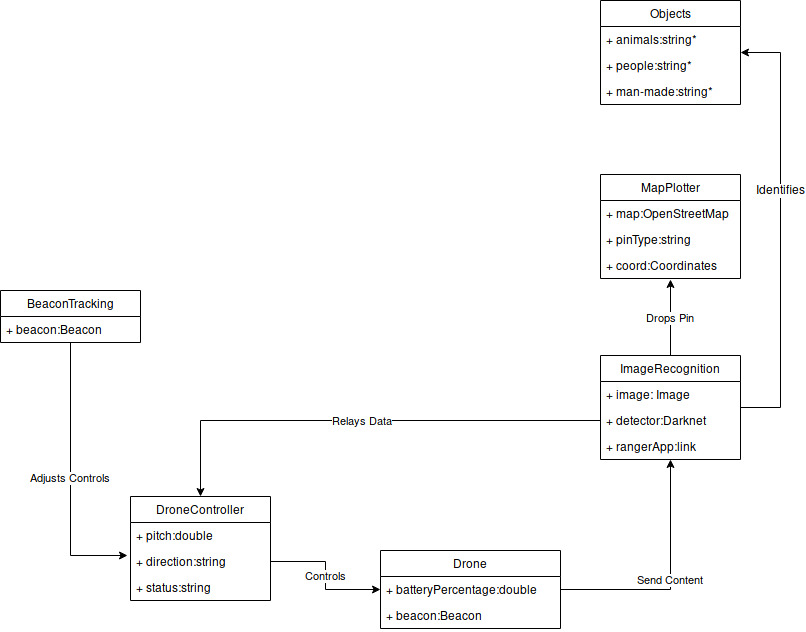
\includegraphics[width=\linewidth]{./assets/images/domain-model.jpg}
	\label{fig: Domain Model}
	\caption{Domain Model}
\end{figure}

% \section{Product Perspective}
% $<$Describe the context and origin of the product being specified in this SRS.
% For example, state whether this product is a follow-on member of a product
% family, a replacement for certain existing systems, or a new, self-contained
% product. If the SRS defines a component of a larger system, relate the
% requirements of the larger system to the functionality of this software and
% identify interfaces between the two. A simple diagram that shows the major
% components of the overall system, subsystem interconnections, and external
% interfaces can be helpful.$>$

% \section{Product Functions}
% $<$Summarize the major functions the product must perform or must let the user
% perform. Details will be provided in Section 3, so only a high level summary
% (such as a bullet list) is needed here. Organize the functions to make them
% understandable to any reader of the SRS. A picture of the major groups of
% related requirements and how they relate, such as a top level data flow diagram
% or object class diagram, is often effective.$>$

\section{User Classes and Characteristics}

\begin{flushleft}
	A typical user of the system is characterised as an employee (volunteer) of ERP. 
	These employees can be divided into two main classes:
	\newline
	\newline
	\textbf{Ranger:}
	\newline
	% TODO: Add citation
	The ranger is a person entrusted with protecting and preserving the wildlife park. 
	The FMDS will be used as an augmentation to the current ranging procedures. 
	The ranger needs to be technology savvy to use the system.
	It is necessary that the ranger knows how to operate a mobile device ie.\ phone/tablet.
	This is an essential part of controlling the drone with regard to take off, initiating flight patterns and landing procedures.
	\newline
	\newline
	\textbf{Command Centre Personnel:}
	\newline
	Command center personnel are employees with specialized skills to analyze data collected during the time the drone is airborne. 
	Data to be analyzed includes mapping data and new footage for further training of the object recognition.
	
	
\end{flushleft}
% $<$Identify the various user classes that you anticipate will use this product.
% User classes may be differentiated based on frequency of use, subset of product
% functions used, technical expertise, security or privilege levels, educational
% level, or experience. Describe the pertinent characteristics of each user class.
% Certain requirements may pertain only to certain user classes. Distinguish the
% most important user classes for this product from those who are less important
% to satisfy.$>$

\section{Operating Environment}

% $<$Describe the environment in which the software will operate, including the
% hardware platform, operating system and versions, and any other software
% components or applications with which it must peacefully coexist.$>$

The operating environment for the FMDS is listed below: 
\begin{itemize} 
	\item Device - Raspberry Model 3B+
	\item OS - Rasbian 9 (Strech) 
	\begin{itemize}
		\item Linux Kernel v14.4
		\item gcc v6.3
		\item apt v1.4.9
	\end{itemize}
	\item Camera - Raspberry Pi Camera Module V2.8 1080p
\end{itemize}



% \section{Design and Implementation Constraints}
% $<$Describe any items or issues that will limit the options available to the
% developers. These might include: corporate or regulatory policies; hardware
% limitations (timing requirements, memory requirements); interfaces to other
% applications; specific technologies, tools, and databases to be used; parallel
% operations; language requirements; communications protocols; security
% considerations; design conventions or programming standards (for example, if the
% customer’s organization will be responsible for maintaining the delivered
% software).$>

% \section{User Documentation}
% $<$List the user documentation components (such as user manuals, on-line help,
% and tutorials) that will be delivered along with the software. Identify any
% known user documentation delivery formats or standards.$>$
% \section{Assumptions and Dependencies}

% $<$List any assumed factors (as opposed to known facts) that could affect the
% requirements stated in the SRS. These could include third-party or commercial
% components that you plan to use, issues around the development or operating
% environment, or constraints. The project could be affected if these assumptions
% are incorrect, are not shared, or change. Also identify any dependencies the
% project has on external factors, such as software components that you intend to
% reuse from another project, unless they are already documented elsewhere (for
% example, in the vision and scope document or the project plan).$>$
